\subsection{The Boot Process}
\label{sec:booting}

When a computer is powered up, it undergoes a \textit{bootstrapping} process,
also called \textit{booting}, for simplicity. Although many steps in the boot
process depend on the motherboard and components in a computer, the process
does follow a high-level structure that is mostly prescribed in the SDM. This
section provides the details needed to analyze SGX's security properties.
\cite{intel2010booting} provides a good reference on the low-level details of
the entire booting process.

\subsubsection{UEFI Platform Initialiaztion}
\label{sec:efi}

The firmware in recent computers with Intel processors implements the
\textit{Platform Initialization} (PI) process in the \textit{Unified
Extensible Firmware Interface} (UEFI) specification \cite{forum2015uefi}. The
platform initialization follows the steps shown in Figure~\ref{fig:uefi} and
described below.

\begin{figure}[hbt]
  \center{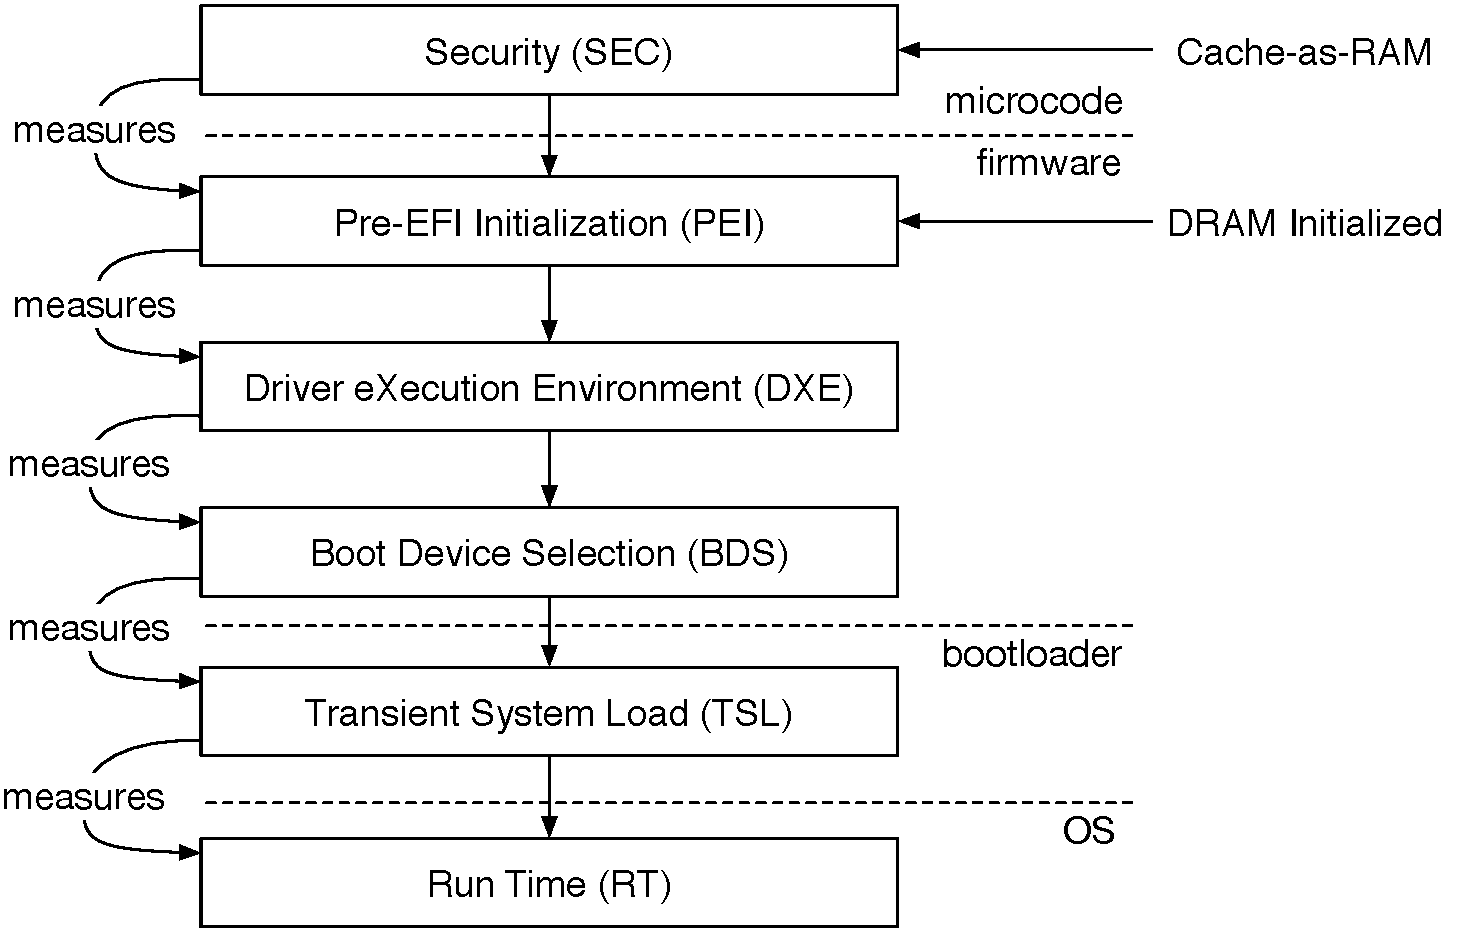
\includegraphics[width=85mm]{figures/uefi.pdf}}
  \caption{
    The phases of the Platform Initialization process in the UEFI
    specification.
  }
  \label{fig:uefi}
\end{figure}

The computer powers up, reboots, or resumes from sleep in the
\textit{Security phase} (SEC). The SEC implementation is responsible for
establishing a temporary memory store and loading the next stage of the
firmware into it. The SEC implementation also performs any security-related
tasks, such as measuring (computing a cryptographic hash of) the next firmware
stage, and potentially aborting if the firmware is not signed by a pre-approved
key.

SEC is followed by the \textit{Pre-EFI Initialization phase} (PEI), which
initializes the computer's DRAM, copies itself from the temporary memory
store into DRAM, and tears down the temporary storage. When the computer is
powering up or rebooting, the PEI implementation is also responsible for
initializing all the non-volatile storage units that contain UEFI firmware and
loading the next stage of the firmware into DRAM. When recovering from sleep

PEI hands off control to the \textit{Driver eXecution Environment phase} (DXE).
In DXE, a loader locates and starts firmware drivers for the various components
in the computer. DXE is followed by a Boot Device Selection (BDS) phase, which
is followed by a Transient System Load (TSL) phase, where an EFI application
loads the operating system selected in BDS. Last, the OS loader passes control
to the operating system's kernel, entering the Run Time (RT) phase.

On a system that uses secure boot or attestation, the SEC implementation is the
system's root of trust. Each platform initialization phase is responsible for
verifying or measuring the firmware that implements next phase. For example, in
a TPM / TXT system, SEC firmware initializes the TPM registers that hold the
system's measurement, which are the Platform Configuration Registers (PCRs) for
the Static Root of Trust Measurement (SRTM). The SEC implementation then stores
the PEI's measurement (cryptographic hash) into a measurement register. In
turn, the PEI implementation measures the DXE firmware and updates the
measurement register that stores the PEI hash to account for the DXE hash. When
the OS is booted, the hash in measurement register accounts for all the
firmware that was used to boot the computer.


\subsubsection{SEC on Intel Platforms}
\label{sec:uefi_sec_details}

% Initialization Overview: SDM S 9.1

The SEC phase starts in the CPU's circuitry. Right after a computer is powered
up, all the logical processors (LPs) on the motherboard undergo
\textit{hardware initialization}, which invalidates the caches
(\S~\ref{sec:caching}) and TLBs (\S~\ref{sec:tlbs}), performs a
\textit{Built-In Self Test} (BIST), and sets all the registers
(\S~\ref{sec:registers}) to pre-specified values.

% Multiple-Processor Initialization: SDM S 8.4
% BSP and AP Processors: SDM S 8.4.1
% MP Initialization Protocol Algorithms for MP Systems: SDM S 8.4.3
% An Ivy Bridge CPUID: family 06h, extended model 3, model 58, stepping 9

After hardware initialization, the LPs perform the Multi-Processor (MP)
initialization algorithm, which results in one LP being selected as the
\textit{bootstrap processor} (BSP), and all the other LPs being classified as
\textit{application processors} (APs).

According to the SDM, the details of the MP initialization algorithm for recent
CPUs depend on the motherboard and firmware. In principle, after completing
hardware initialization, all LPs attempt to issue a special no-op transaction
on the QPI bus. A single LP will succeed in issuing the no-op, thanks to
the QPI arbitration mechanism, and to the UBox (\S~\ref{sec:cache_coherence})
in each CPU package, which also serves as a ring arbiter. The arbitration
priority of each LP is based on its APIC ID (\S~\ref{sec:interrupts}), which is
provided by the motherboard when the system powers up. The LP that issues the
no-op becomes the BSP. Upon failing to issue the no-op, the other LPs become
APs, and enter the \textit{wait-for-SIPI} state.

% Typical BSP Initialization Sequence: SDM S 8.4.4.1

Understanding the PEI firmware loading process is unnecessarily complicated by
the fact that the SDM describes a legacy process consisting of having the BSP
set its RIP register to 0xFFFFFFF0 (16 bytes below 4GB), where the firmware is
expected to place a instruction that jumps into the PEI implementation.

% FIT pointer is at 4GB - 0x18.
%   US 8,429,418 - 3:52-55, Fig 4
%   US 8,321,931 - Fig 5, 12:34-39

Recent processors do not support the legacy approach at all
\cite{reinauer2013fitpatch}. Instead, the BSP reads a word from address
0xFFFFFFE8 (24 bytes below 4GB) \cite{intel2012uefihypervisor, datta2013acm},
and expects to find the address of a \textit{Firmware Interface Table} (FIT)
in the memory address space (\S~\ref{sec:address_spaces}), as shown in
Figure~\ref{fig:firmware_fit}. The BSP is able to read firmware contents from
non-volatile memory before the computer is initialized, because the initial SAD
(\S~\ref{sec:cache_coherence}) and PCH (\S~\ref{sec:motherboard})
configurations maps a region in the memory address space to the SPI flash chip
(\S~\ref{sec:motherboard}) that stores the computer's firmware.

\begin{figure}[hbt]
  \center{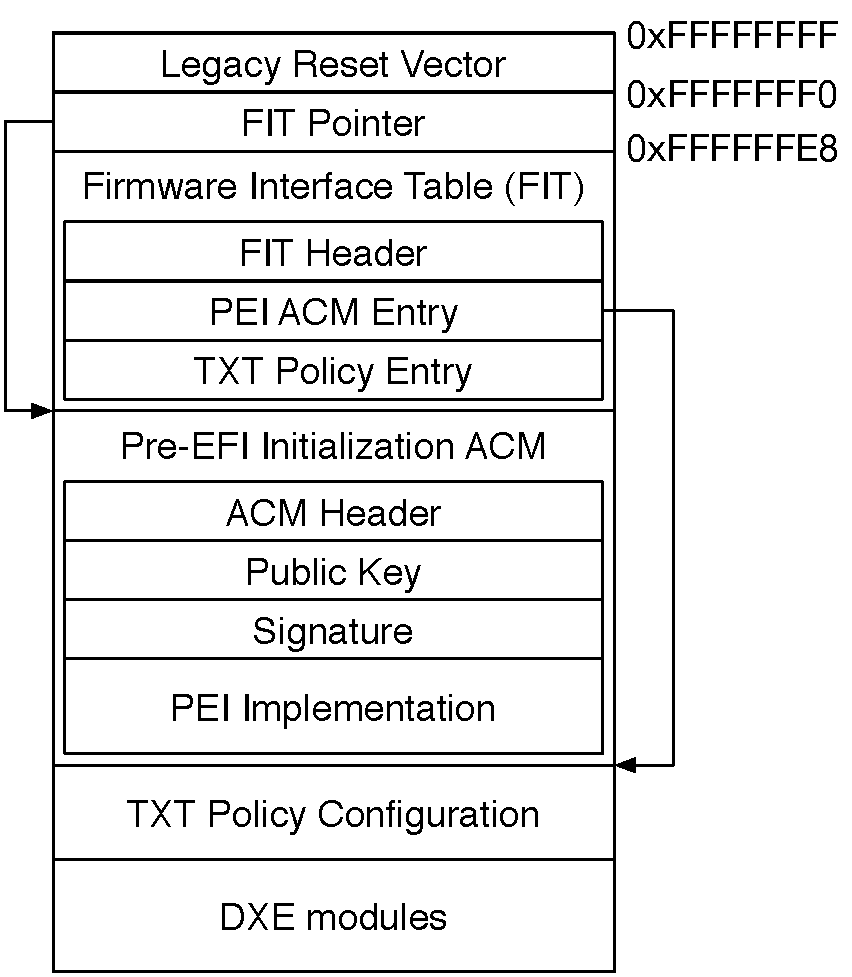
\includegraphics[width=55mm]{figures/firmware_fit.pdf}}
  \caption{
    The Firmware Interface Table (FIT) in relation to the firmware's memory
    map.
  }
  \label{fig:firmware_fit}
\end{figure}

The FIT \cite{qureshi2006fit} was introduced in the context of Intel's Itanium
architecture, and its use in Intel's current 64-bit architecture is described
in an Intel patent \cite{datta2013acm} and briefly documented in an obscure
piece of TXT-related documentation \cite{intel2010txtlab}. The FIT contains
\textit{Authenticated Code Modules} (ACMs) that make up the firmware, and
other platform-specific information, such as the TPM and TXT configuration
\cite{intel2010txtlab}.

The PEI implementation is stored in an ACM listed in the FIT. The processor
loads the PEI ACM, verifies the trustworthiness of the ACM's public key, and
ensures that the ACM's contents matches its signature. If the PEI passes the
security checks, it is executed. Processors that support Intel TXT only accept
Intel-signed ACMs \cite[p. 92]{futral2013servertxt}.


\subsubsection{PEI on Intel Platforms}
\label{sec:uefi_pei_details}

\cite{intel2010booting} and \cite{coreboot2015manual} describe the
initialization steps performed by Intel platforms during the PEI phase, from
the perspective of a firmware programmer. A few steps provide useful context
for understanding SGX's hardware underpinnings.

% Preventing Caching: SDM S 11.5.3

When the BSP starts executing PEI firmware, DRAM is not yet initialized.
Therefore the PEI code starts executing in a \textit{Cache-as-RAM} (CAR) mode,
which only relies on the BSP's internal caches, at the expense of imposing
severe constraints on the size of the PEI's working set.

One of the first tasks performed by the PEI implementation is enabling DRAM,
which requires discovering and initializing the DRAM chips connected to the
motherboard, and then configuring the BSP's memory controllers
(\S~\ref{sec:cache_coherence}) and MTRRs (\S~\ref{sec:memory_io}). Most
firmware implementations use Intel's \textit{Memory Reference Code} (MRC) for
this task.

After DRAM becomes available, the PEI code is copied into DRAM and the BSP is
taken out of CAR mode. The BSP's LAPIC is initialized and used to send a
broadcast \textit{Startup Inter-Processor Interrupt} (SIPI) to wake up the
APs. The interrupt vector in a SIPI indicates the memory address of the AP
initialization code in the PEI implementation.

% Typical AP Initialization Sequence: SDM S 8.4.4.2

The PEI code responsible for initializing APs is executed when the APs receive
the SIPI wake-up. The AP PEI code sets up the AP's configuration registers,
such as the MTRRs, to match the BSP's configuration. Next, each AP registers
itself in a system-wide table, using a memory synchronization primitive, such
as a semaphore, to avoid having two APs access the table at the same time.
After the AP initialization completes, each AP is suspended again,
and waits to receive an INIT Inter-Processor Interrupt from the OS kernel.

The BSP initialization code waits for all APs to register themselves into the
system-wide table, and then proceeds to locate, load and execute the firmware
module that implements DXE.
